%!TEX root = ../template.tex
%%%%%%%%%%%%%%%%%%%%%%%%%%%%%%%%%%%%%%%%%%%%%%%%%%%%%%%%%%%%%%%%%%%%
%% chapter3.tex
%% NOVA thesis document file
%%
%% Planning Chapter
%%%%%%%%%%%%%%%%%%%%%%%%%%%%%%%%%%%%%%%%%%%%%%%%%%%%%%%%%%%%%%%%%%%%

\typeout{NT FILE chapter3.tex}%

\chapter{Planning}
\label{cha:Planning}

\section{Proposed Timeplan and Workflow}
In this chapter, a time-plan to be followed during the course of this
dissertation is proposed(figure \ref{fig:timeplan}), with a brief description
of each step being presented afterwards.

\begin{figure}[htbp]
	\centering
	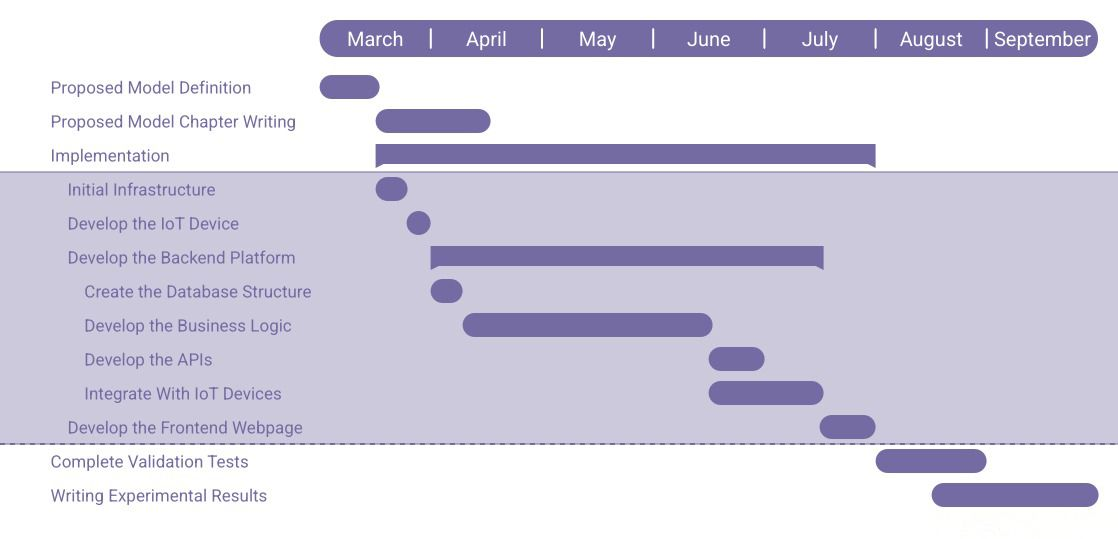
\includegraphics[width=\textwidth]{Chapters/Figures/Planning/Planning.jpeg}
	\caption{Gantt chart with the proposed timeplan}
	\label{fig:timeplan}
\end{figure}

\begin{description}
	\item[Proposed Model Definition:] The system's architecture will be designed
	      over the first half of March. The general structure will be defined as
	      well as each component's tech stack and how they communicate.
	\item[Proposed Model Chapter Writing:]  After the model has been established,
	      the proposed model's chapter will be written, describing the architecture
	      in depth as well as its inner components.
	\item[Implementation:] Between the second half of March and July, the defined model will be
	      implemented. During this phase, each component will be developed as designed
	      and tested. Firstly, the basic infrastructure of the defined
	      architecture will be configured, then, a simple \gls{IoT} device will
	      be developed. Between April and half of July, the backend platform
	      will be developed, starting by creating the database structure
	      previously designed, then, during the next two months, the business
	      logic will be developed, and finally, after that the \gls{API} will be
	      created to integrate with the \gls{IoT} device and frontend. In the
	      last half of July, the frontend web platform will be developed as
	      proof of concept.
	      The testing will be done both by unit (unit testing) and to the
	      integration between components (integration testing).
	\item[Complete Validation Tests: ]After the development phase, the whole
	      architecture will be tested and validated over the month of August.
	\item[Writing Experimental Results:] The experimental results will be
	      documented in full in the dissertation in the last two months and
	      the state-of-the-art will be revised.
\end{description}

